\documentclass[conference]{IEEEtran}
\usepackage[]{graphicx}
\graphicspath{ {images/} }
\usepackage{caption}
\usepackage{subcaption}
\usepackage{blindtext, graphicx}
\usepackage{amsmath}

% correct bad hyphenation here
\hyphenation{op-tical net-works semi-conduc-tor}

\graphicspath{ {images/} }

\begin{document}

\title{Classifying Dysarthria Patients with Long Short-Term Memory Networks}

\author{\IEEEauthorblockN{Alex Mayle}
\IEEEauthorblockA{School of EECS \\
Ohio University \\
am218112@ohio.edu}}

\maketitle

\begin{abstract}
This paper presents a recurrent neural network architecture for the binary classification of Mandarin speaking individuals into two classes, those who are afflicted with some form of Dysarthria, and those who are not. Specifically, a series of Long Short-Term Memory (LSTM) networks are evaluated on the task using accuracy, and the rate of both false positives and negatives as metrics. A double layer, one directional LSTM is shown to slightly outperform the others, and significantly improve upon a baseline Multi-layer Perceptron  employed for the same task. While the results are not indicative of a practical replacement for a medical diagnosis, we show that the LSTM's ability to leverage temporal information from within its inputs makes for an effective step in the pursuit of accessible Dysarthria diagnoses. 
\end{abstract}

\section{Introduction}
There are approximately 7 million individuals in China suffering from various speech disabilities. One such disorder, Dysarthria, results in an increased difficulty to articulate phonemes, or that which distinguishes one word from another. The impact of Dysarthria is exacerbated in Mandarin speaking individuals due to the fact that variations in tone have the potential to carry different meanings. Given the amount of Chinese speakers suffering from this particular disease, and the challenges it poses to effective communication, accessible means to a diagnosis is paramount. To this end, we present a collection of Recurrent Neural Network (RNN) architectures capable of discerning those who suffer from Dysarthria, given Mandarin syllable pronunciations as input. 

While there are established medical practices regarding the diagnosis of Dysarthria, such as the Frenchay Dysarthria Assessment \cite{enderby1980frenchay}, such techniques require the patient be physically present and undergo a series of examinations. In contrast, the system presented here increases accessibility by merely relying on speech as input. While it's doubtful that such a system can completely replace a diagnosis by a medical practitioner, it has the potential to provide a more accessible, less invasive, first step in seeking care. 

We present a collection of Long Short-term Memory (LSTM) architectures and evaluate them through several experiments. First, we conduct a baseline experiment to test if LSTM networks provide an advantage over non-recurrent models. The recurrent networks are then evaluated on several variants of the data set to gain insight into the most effective inputs for dysarthria classification.

\section{Model}
Given an audio clip $X$, containing the pronunciation of a Mandarin syllable, the model is to produce a label $Y$ indicating whether or not the speaker suffers from Dysarthria. We refer to a positive result as a diagnosis of Dysarthria. The raw waveform $X$ is first transformed into an MFCC feature vector $X' = \{x_1, x_2,...x_t\}$, where $t$ is dependent on the length of $X$. Each element of $X'$ is then fed into a LSTM network sequentially. After $x_t$ has been input, the LSTM network produces the vector $h_t$, which is then used as input to logistic regression. Finally, the regression layer outputs the aforementioned label $Y$.  Figure \ref{fig-architecture} illustrates a single training example's path through the network. 

\subsection{Pre-processing}
We began by transforming the raw audio $X$ into an MFCC feature vector $X'$ using a sliding window of $25$ milliseconds and a $10$ millisecond stride. Each MFCC in $X' = \{x_1, x_2,...x_t\}$ consists of $n$ coefficients $x_i = \{\theta_1...\theta_{n}\}$, where $n = 13$ unless explicitly stated. In practice, the network is trained on many such inputs $X$. These were collected and normalized such that the $k$th coefficient $\theta_k$ had zero-mean and unit variance with respect to $\theta_k$ across all training examples. 

Since each input $X'$ contains a varying amount of MFCC's, each mini-batch fed into the network is $0$-padded such that each $X'$ in the mini-batch has the same length $t_{max}$, where $t_{max}$ is the largest $t$ value in the mini-batch. However, we do keep track of the lengths of each $X'$ and instruct the LSTM network not to process the padded portion of each input $X'$. That is, the LSTM runs $t$ time steps for each input $X' = \{x_1, x_2,...x_t, 0_{t+1}, ..., 0_{t_{max}}\}$ in the mini-batch.

\subsection{LSTM Architecture}
After pre-processing, $X'$ is then fed into a LSTM network. As noted, because $X'$ is a time-series of MFCC's, we do not input them concurrently. Instead, we feed in one MFCC each time-step. The network produces an output $h_i$ at each time step, but only the last output $h_t$ is used as input to the logistic regression layer. The model is implemented to copy the output from the last non-zero-padded input $h_t$ to $h_{t_{max}}$. In doing so, we guarantee that the output sent to the logistic regression layer is not affected by the zero-padding.

We experimented with several variants of the LSTM model, including adding layers and using a bidirectional LSTM. For the models with one layer, $L2$ regularization was used. The two-layer model employed dropout \cite{Srivastava:2014:DSW:2627435.2670313} between the LSTM layers, as well as between the last LSTM layer and logistic regression. Dropout is never applied between the time-steps, as suggested by Zaremba et al \cite{DBLP:journals/corr/ZarembaSV14}. 

The standard LSTM model is able to use inputs from arbitrarily distant time steps to change its output at the current time step \cite{gers2002learning}. However, it cannot use information from subsequent time steps to affect previous ones. Bidirectional LSTM networks overcome this limitation by performing two concurrent passes on the data. One pass starts from step $0$ to $t$ as normal, while another pass starts at time step $t$ and ends at step $0$. Each pass produces an output, which we handle by concatenating them together and feeding them to the logistic regression layer.

\begin{figure}[t]
\centering
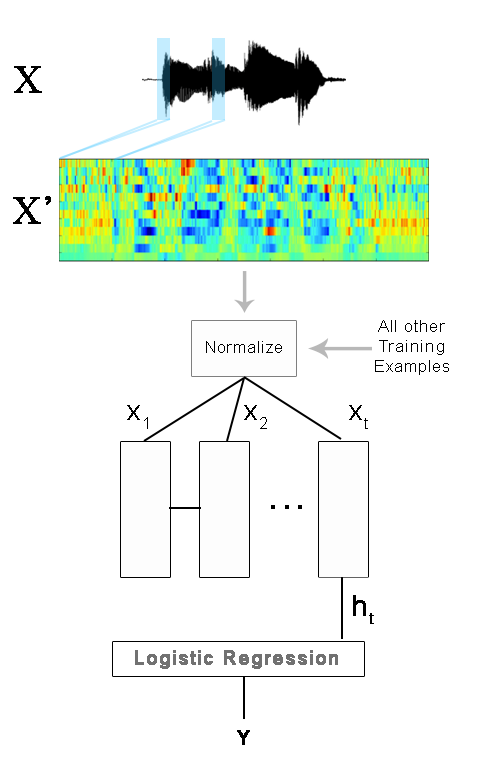
\includegraphics[width=\columnwidth]{architecture}
\caption{A single training example, $X$, as it flows through the network: The input is first converted to $X'$, a variable length MFCC vector of length $t$. It is then normalized with respect to the entire training dataset. Finally, each MFCC in $X'$ is input to the LSTM network sequentially. The final output $h_t$ is fed to the logistic regression layer to produce the label $Y$, indicating whether or not the speaker is afflicted with Dysarthria.}
\label{fig-architecture}
\end{figure}

\section{Methodology}

The data consists of Mandarin speaking adult men and women, where some are afflicted with Dysarthia and others are not. The breakdown of these partitions is presented in Table \ref{tab-data-partitions}.

\begin{table}[h]
\centering
\caption{Data Set}
\label{tab-data-partitions}
\begin{tabular}{|l|c|c|c|}
\hline
\multicolumn{1}{|c|}{}  & Female   &   Male    &    Ratio       \\ \hline
Healthy                 & 1600    &   1605     &    53.4\%      \\ \hline
Patient                 & 1001    &   1792     &    46.6\%      \\ \hline
Total                   & 2601    &   3397     &    100\%       \\ \hline
\end{tabular}
\end{table}

In total, four models are tested, including a baseline model in the first experiment.

\begin{enumerate}
    \item Baseline: multi-layer Perceptron (MLP) consisting of one hidden layer that is fed into the logistic regression classifier.
    \item LSTM-1: Single layer, one-directional LSTM starting from time step 0
    \item LSTM-2: Double layer, one-directional LSTM starting from time step 0
    \item Bi-LSTM-1: Single layer, bi-directional LSTM involving two concurrent passes of the training example. One starting from time step 0, and the other starting at time step $t$. 
\end{enumerate}

They all use a relatively small hidden state size of 200. Because each LSTM cell has four "banks" of parameters, each cell adds 800 parameters to the model. Meaning each model has 400, 1000, 1800, and 1800 parameters, respectively. While $Bi-LSTM-1$ has only one LSTM layer, it does two concurrent passes on the data using two different LSTM cells, giving it the same amount of parameters as $LSTM-2$. 

All models were trained using Adam gradient descent \cite{DBLP:journals/corr/KingmaB14} to minimize the cross entropy between the predictions of the network and the ground truth provided by the medical practitioners who collected the data. Training occurred for 40 epochs on mini-batches of size sixty-four. 

A form of early stopping was employed. Training is cut short when the ration between the current validation error $\epsilon_curr = 1 - f1_curr$ and lowest error seen thus far $\epsilon_min = 1 - f1_max$ exceeds a threshold $/alpha$. A grace period is used, such that training is only stopped if the following condition is met five times without a new minimum error. 

$$ \alpha < \frac{\epsilon_curr}{\epsilon_min} - 1$$,
where $\alpha = 7.5\%$.

\section{Experiment I: Baseline}
We first compare the LSTM models against a baseline MLP on the relatively easy task of non-novel speakers. Meaning, we group the data set such that, for a particular speaker, it is possible for some of their syllables to appear in the training set, while others are in the test set. Specifically, we randomly assign each example in the data set to the training, testing, and validation sets with a ratio of 2:1:1. 

We employ the accuracy, precision, and recall \cite{torgo2009precision} as metrics to judge the performance of each model. Precision and recall are considered due to the medical nature of these experiments. That is, most people do not suffer from dysarthria, but it is the instances in which one does that are important to classify correctly. We therefore define a metric to measure the chance that a dysarthria patient will receive a negative result $FN = 1 - recall$. In an analogous fashion, we define a metric for false-positives $FP = 1 - precision$. Because individuals who receive a negative prediction (i.e., they do not suffer from dysarthria) are less likely to seek a second opinion, we are especially interested in the minimization of $FN$. 

\begin{table}[h]
\centering
\caption{Experimental results}
\begin{tabular}{|l|c|c|c|}
\hline
\multicolumn{1}{|c|}{}    &   Accuracy     &   FP         &     FN         \\ \hline
Baseline                    &   80.1\%     &   -          &     -           \\ \hline
LSTM-1                      &   88.7\%     &   11.5\%     &     8.8\%       \\ \hline
LSTM-2                      &   88.7\%     &   12.0\%     &     8.3\%       \\ \hline
Bi-LSTM-1                   &   87.8\%     &   13.4\%     &     8.2\%      \\ \hline
\end{tabular}
\label{tab-exp-1-results}
\end{table}

Table \ref{tab-exp-1-results} depicts the results for each experiment. Given that the majority classifier would achieve an accuracy of about $53\%$, the baseline is a significant improvement. Moreover, LSTM-1 and LSTM-2 achieve similar performance, beating the baseline and making a marginal improvement upon the Bi-LSTM-1 model.

\begin{figure}[h]
\centering
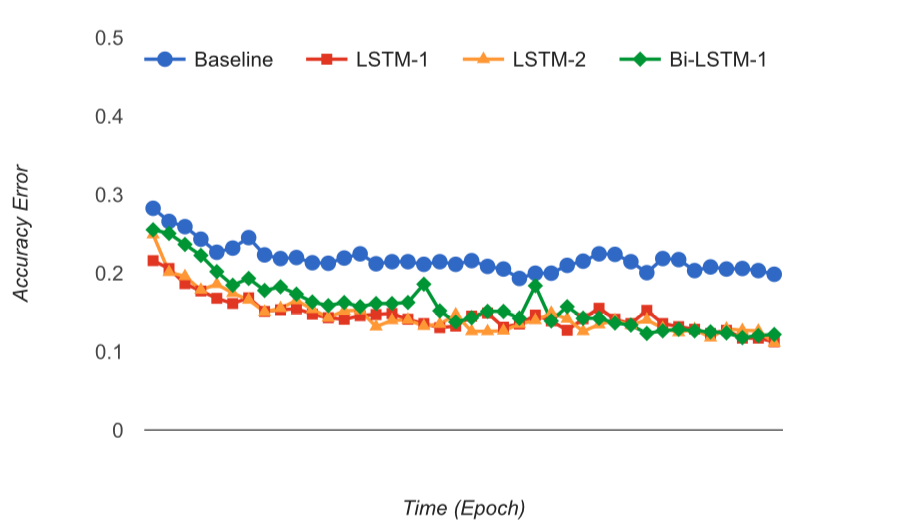
\includegraphics[width=\columnwidth]{convergence}
\caption{Error rate over the 40 epochs of training. The three LSTM models start training with slightly different error rates, but all  eventually converge to a rate superior to the baseline. }
\label{fig-convergence}
\end{figure}

Figure \ref{fig-convergence} shows the accuracy convergence of each model. The LSTM's clearly outperform the baseline; however, increasing the expressive capacity through adding layers and passes over the data did not result in significant performance improvements. LSTM-1 and LSTM-2 achieved the same accuracy, with the latter improving upon the false negatives metric. Because adding a layer resulted in the same performance, and adding another pass was slightly detrimental, we did not consider a two-layer bidirectional model. 

LSTM-2's $88.7$\% accuracy and 8.2\% false negative rate constitute a promising attempt at classifying dysarthria among both afflicted and healthy speakers, but it is important to remember the practical application of these models. When such a system attempts to classify an individual, it has likely never been trained on any of their data. While it is clear that the LSTM models outperform the baseline, we are more interested in how they perform when evaluating novel speakers. 
\section{Experiment II: Novel Speakers}
The first experiment used training and test partitions where a speaker's syllables may appear in both. To more accurately match the potential application, the models in this experiment were tested on novel speakers; an individual's syllables appeared in either the test or train set, but not both. 

Because the number of speakers in the data set is small, at sixty-nine, we opted to evaluate the models using a 10-fold cross validation. Nine of the speakers were randomly set aside as a validation set. We then partitioned the remaining sixty into ten groups of six. A cross validation trial consisted of ten rounds, distinguished by which fold is used as the test set. Meaning, in each round, the models were trained on fifty-four speakers and tested on a set of six novel speakers.

The prior experiment effectively rounded the logistic regression layer's activation to produce the label $Y$. In contrast, the following experiments consider three ways to interpret the activations: syllable, soft-majority, and noisy-OR. The first is simply the un-transformed output from the logistic regression layer $\alpha_{reg}$, when given a single syllable. In contrast, the latter two methods consider all of a speakers' examples. Rather than classifying a syllable, soft-majority and noisy-OR classify a speaker. 

Because the traditional nosiy-OR calculation would be affected by the number of syllables each speaker has, we computed it in log-space and normalized by the number of syllables in the calculation. This allowed us to directly compare the nosy-OR scores between speakers with a varying number of examples.

For the logistic regression activations for all of some speaker's syllables $\{\alpha_{reg}^{(0)}, \alpha_{reg}^{(1)},...,\alpha_{reg}^{(m-1)}\}$ and some integer $k \in [0,m-1]$,

\begin{align}
syllable &= \alpha_{reg}^{(k)},\\
soft-majority &= \frac{1}{m} \sum_{i=0}^{m-1} \alpha_{reg}^{i} \\
noisy-OR &= \frac{1}{m} \sum_{i=0}^{m-1} log(1-\alpha_{reg}^{i})
\end{align}

\ref{fig-exp-2-results} presents the receiver-operator and precision-recall curves for each method of inference while \ref{tab-exp-2-results} lists their respective area under curve (AUC) scores. The soft-majority and noisy-OR methods produced identical results, so the latter's curve is not explicitly shown. 

To gain perspective on these AUC scores, we consider a model which produces a positive classification with probability $\theta$. The majority classifier can be seen as the extreme case, where $\theta = 1$. As $\theta$ increases from $0$ to $1$, the red linear curve in \ref{fig-exp-2-results} is produced. Graphically, we can see that the AUC of this curve is $.5$. 

The models clearly improve upon this baseline for all three methods of inference. Moreover, while all three LSTMs performed similarly in the first experiment, $LSTM-1$ clearly produces the most impressive results on novel speakers. 

As expected, soft-majority and noisy-OR achieved higher scores than syllable level evaluation. It is worth pointing out that these two methods' are more appropriate for practical purposes; we would be remiss to think that an accurate diagnosis could result from a single syllable. 

\begin{table}[h]
\centering
\caption{Experimental results}
\begin{tabular}{|l|c|c|c|}
\hline
\multicolumn{1}{|c|}{}    &   Syllable     &   Soft-Majority         &     Fuzzy-Or         \\ \hline
LSTM-1                      &   .754     &   .854     &     .854       \\ \hline
LSTM-2                      &   .695     &   .785     &     .785       \\ \hline
Bi-LSTM-1                   &   .714     &   .847     &     .847      \\ \hline
\end{tabular}
\label{tab-exp-2-results}
\end{table}


\begin{figure*}[t]
    \centering
    \begin{subfigure}[b]{0.4\textwidth}
        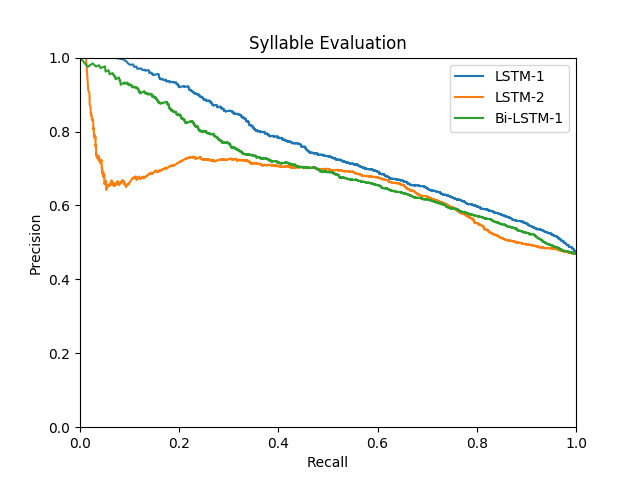
\includegraphics[width=\textwidth]{syl_pr}
        \caption{}
        \label{rfidtest_xaxis}
    \end{subfigure}
    \begin{subfigure}[b]{0.4\textwidth}
        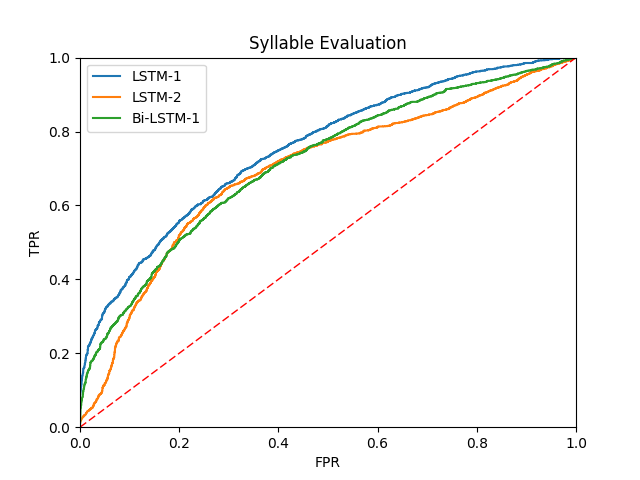
\includegraphics[width=\textwidth]{syl_roc}
        \caption{}
        \label{rfidtest_yaxis}
    \end{subfigure}
    \begin{subfigure}[b]{0.4\textwidth}
        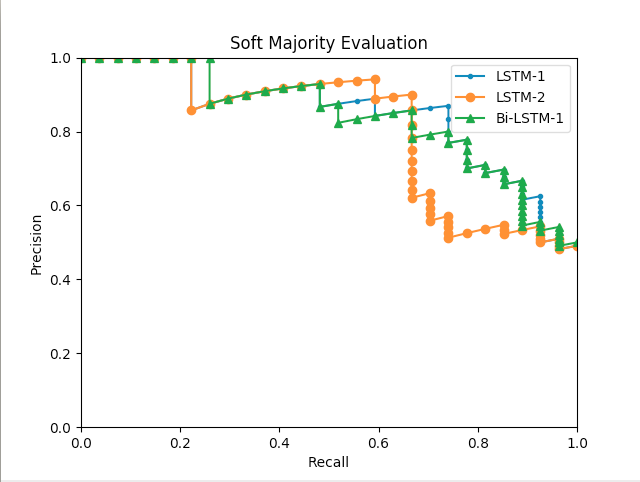
\includegraphics[width=\textwidth]{sm_pr}
        \caption{}
        \label{rfidtest_zaxis}
    \end{subfigure}
    \begin{subfigure}[b]{0.4\textwidth}
        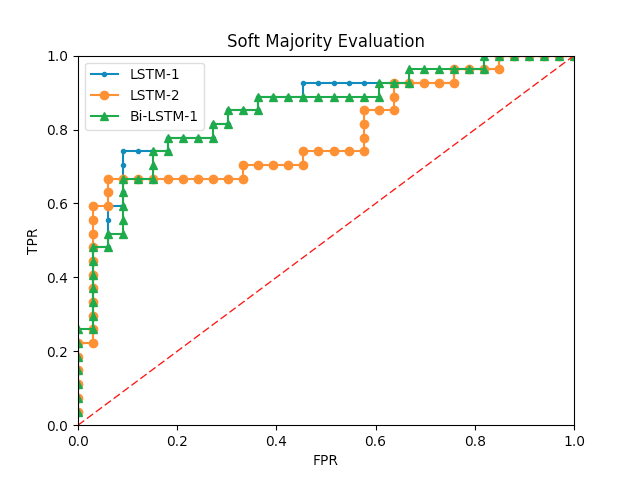
\includegraphics[width=\textwidth]{sm_roc}
        \caption{}
        \label{rfidtest_zaxis}
    \end{subfigure}
    \caption[]{}
    \label{fig-exp-2-results}
\end{figure*}

\section{Varying Cepstrum Coefficients}
While including thirteen cepstrum coefficients in each feature has produced promising results, there may still be room for improvement by adding additional coefficients. We created a new data set with twenty-five coefficients in each feature. Three ten fold validation trials were conducted in the same manner as experiment II, with thirteen, nineteen, and all twenty-fave coefficients used as input, respectively. When all of them are not included in each feature, the coefficients are taken starting from the cepstrum with the lowest quefrency. We report the AUC score for each model using their soft-majority predictions.

\begin{table}[h]
\centering
\caption{Experimental results}
\begin{tabular}{|l|c|c|c|}
\hline
\multicolumn{1}{|c|}{}      &   13         &   19         &     25           \\ \hline
LSTM-1                      &   84.2     &   90.1     &     81.7       \\ \hline
LSTM-2                      &   79.1     &   88.2     &     87.1       \\ \hline
Bi-LSTM-1                   &   84.9     &   88.4     &     90.4       \\ \hline
\end{tabular}
\label{tab-results}
\end{table}

\begin{figure*}[t]
    \centering
    \begin{subfigure}[b]{0.4\textwidth}
        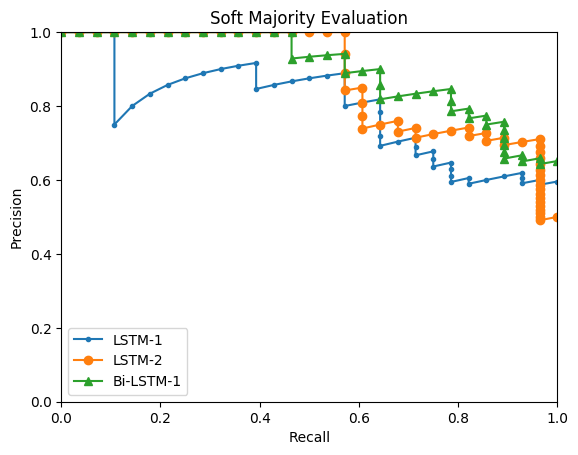
\includegraphics[width=\textwidth]{25cep-sm-pr.png}
        \caption{}
        \label{rfidtest_xaxis}
    \end{subfigure}
    \begin{subfigure}[b]{0.4\textwidth}
        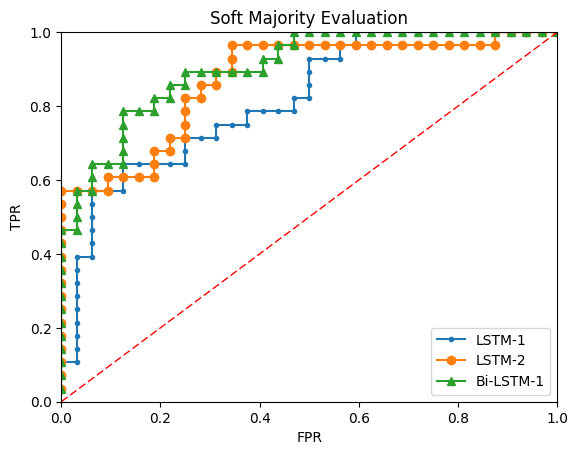
\includegraphics[width=\textwidth]{25cep-sm-roc.png}
        \caption{}
        \label{rfidtest_yaxis}
    \end{subfigure}
    \begin{subfigure}[b]{0.4\textwidth}
        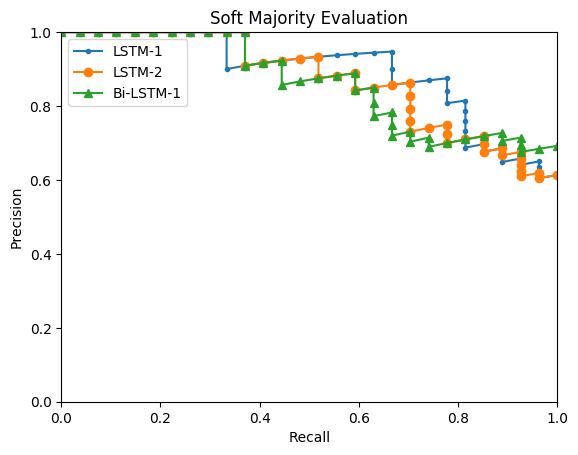
\includegraphics[width=\textwidth]{19cep-sm-pr.png}
        \caption{}
        \label{rfidtest_zaxis}
    \end{subfigure}
    \begin{subfigure}[b]{0.4\textwidth}
        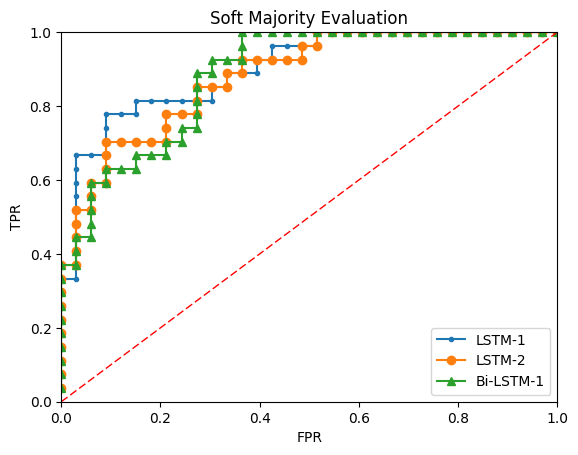
\includegraphics[width=\textwidth]{19cep-sm-roc.png}
        \caption{}
        \label{rfidtest_zaxis}
    \end{subfigure}
    \caption[]{}
    \label{rfidtag_testing}
\end{figure*}

Figure \ref{curves} I need to consolidate this into two graphs, an ROC and PR curve with all six models each.  

The standard thirteen coefficient input produced familiar results, but adding additional information to each feature lead to improved performance in some cases. Interestingly, $LSTM-1$ performed almost as well as $Bi-LSTM-1$ with size nineteen and twenty-five inputs, respectively. However, it seems the opposite is untrue, as $LSTM-1$'s performance decreases when given all of the coefficients as input. Considering it is the smallest model, in terms of parameters, it may be due to a lack of capacity. In general, it seems the models of sufficient size can take advantage of the extra coefficients. 


\section{Syllable types}
Upon evaluating the models in Experiment I, it became clear that they do not perform equally across all classes of syllables. In particular, those prefixed with "z", such as "z-wei", appear to be more difficult for the classifiers. In this experiment, we test how well the models perform when they are trained on a subset of the syllables.

There are three main classes of syllables that appear in the data set: those prefixed with "z", "zz", and those without a prefix. We created two new data sets with the "z" and "zz" syllables filtered out, respectively. We perform a 10 fold cross validation using these filtered sets and present the AUC scores in table \ref{tab-syl-type-results}. 

\begin{table}[h]
\centering
\caption{Experimental results}
\begin{tabular}{|l|c|c|c|c|}
\hline
\multicolumn{1}{|c|}{}      &   None       &   z          &     zz      &    sh       \\ \hline
LSTM-1                      &   84.9     &   92.3    &     62.1  &             \\ \hline
LSTM-2                      &   78.3     &   90.2     &     84.5  &             \\ \hline
Bi-LSTM-1                   &   84.7     &   92.0     &     85.9  &             \\ \hline
\end{tabular}
\label{tab-syl-type-results}
\end{table}

\begin{figure*}[t]
    \centering
    \begin{subfigure}[b]{\columnwidth}
        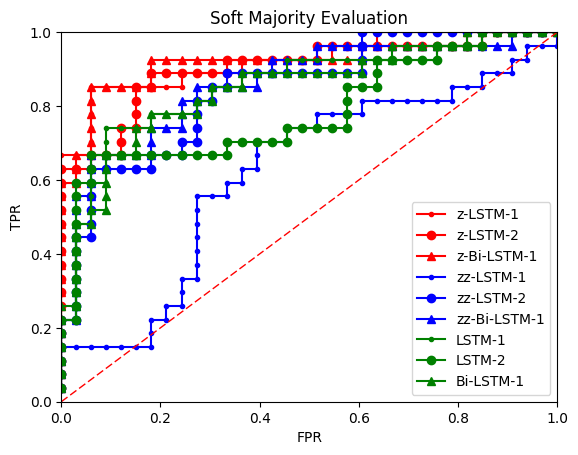
\includegraphics[width=\textwidth]{syl_type_exp-roc.png}
        \caption{}
        \label{rfidtest_xaxis}
    \end{subfigure}
    \begin{subfigure}[b]{\columnwidth}
        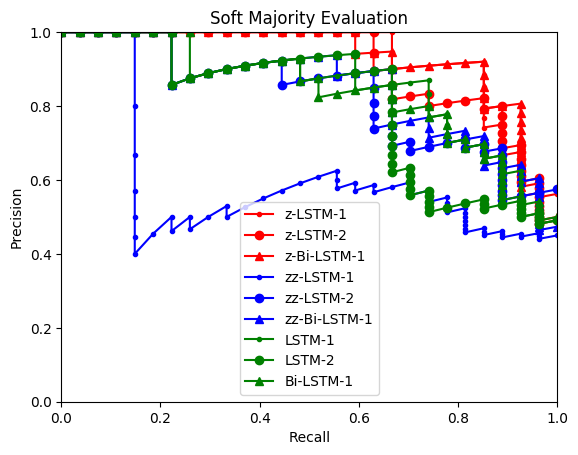
\includegraphics[width=\textwidth]{syl_type_exp-pr.png}
        \caption{}
        \label{rfidtest_yaxis}
    \end{subfigure}
\end{figure*}

Figure \ref{curves} I need to consolidate this into two graphs, an ROC and PR curve with all six models each.  

The models whose input did not include syllables prefixed with "z" performed significantly better according to their AUC scores. Models who were not trained on "zz" prefixed syllables did not fair so well, especially $LSTM-1$. In contrast, $LSTM-2$ improves when "zz" syllables are excluded from its input. 

Both the "z" and "zz" syllables contribute about the same to the number of syllables, at 27 and 76 percent. Being that all three models scored above 90 when trained without "z" syllables, it may be a wise heuristic, especially for smaller data sets such as this. This intuitively follows from the observation that, even for healthy speakers, these syllables are more difficult to pronounce correctly.


To be written
\section{Related Work}
Carmichael et al \cite{carmichael2008combining} employed a multilayer perceptron to classify the different forms of Dysarthria using human speech. Unlike our work, however, the network inputs are assumed to come from a distribution of people known to have some form of Dysarthria. Prior to this, an effort was made to classify speakers into one of the categories of Dysarthria using the Frenchay Dysarthria Assessement of each patient as input \cite{enderby1980frenchay} \cite{carmichael2007introducing}. The more advanced topic of recognizing speech produced from someone with Dysarthria using RNN networks has also been investigated recently \cite{dys-speech-rec-1} \cite{dys-speech-rec-2}. 
\section{Future Work}
ZCA whitening is commonly employed as a pre-processing step in many audio classification tasks \cite{zca-1} \cite{zca-2} \cite{zca-3}. Unfortunately, this proved to be intractable on our implementation machine as the co-variance matrix of the data does not fit in memory. Given the ease of computing the transformation on an appropriate machine, it is a compelling next step in an effort to improve performance. Another technique, batch normalization has also been shown to improve performance \cite{DBLP:journals/corr/CooijmansBLC16}. While we considered implementing this, the level of abstraction with which we define the LSTM model did not provide the necessary level of granularity.

Barring minor improvements made possible by more foresight, we consider architectural additions which may increase performance. The solutions discussed in this paper are monolithic, end-to-end networks. Alternatively, one may use a recursive network structure similar to the one employed in \cite{carmichael2008combining}. Different networks are trained independently, then combined to produce one, larger classifier. For example, one network may classify the speakers' gender or rate of speech first, providing more information to the next layer to use. This pattern would culminate in a final dysarthria classification layer. The model presented in \cite{DBLP:journals/corr/LeePKN17} take features much closer to the raw waveform when compared to MFCCs. Applying this approach to dysarthria classification may also prove to be effective. 
\section{Conclusion}
This paper investigates the effectiveness of LSTM networks in the classification of dysarthria among both afflicted and healthy Mandarin speakers. When presented with a single syllable pronunciation, we found that single and double layer, one-directional LSTM networks slightly outperform their bidirectional single layer counterpart. Further, the double-layer LSTM regularized with dropout between layers exhibit an improvement in the rate of false negatives. While these methods are not yet practical as a standalone medical test, they do suggest that LSTM networks may provide a fruitful avenue for the realization of autonomous dysarthria classification.

\bibliographystyle{unsrt}
\bibliography{references}

\end{document}
